\documentclass{article}
\usepackage{setspace}
\usepackage{natbib}
\usepackage{amsmath}
\usepackage{float}
\usepackage{longtable}
\usepackage{booktabs}
\usepackage{lscape}
\usepackage{graphicx}
\usepackage{silence}
\usepackage{forest}
\usepackage{hyperref}
\usepackage{placeins}
\usepackage{textcomp} % Needed on Windows in Office
\usepackage{adjustbox}
\usepackage{xcolor}
\usepackage[letterpaper, margin=1in]{geometry}

\usepackage[toc,page]{appendix}

\begin{document}
	\subsection{Northeast Alliance}
	\label{sec:Analysis_NEA}
	The first of these areas of investigation is to evaluate the NEA's impact on the offering of codeshare itineraries by JetBlue and American in nonstop markets impacted by the NEA.  
    To analyze this, for origin-destination airport pair $j$ at time $t$,  I estimate the model \[Y_{jt} = \alpha N_{j} + \sum_{T = -8}^{8} \delta_{T} P_{t = T} + \sum_{T = -8, t = 8}^{8} \gamma_{T} N_{j} P_{t = T} + \epsilon_{jt}\] where $Y_{jt}$ is a dummy variable that is 1 if at least one itinerary was recorded was a codeshare itinerary with flights operated by either JetBlue or American and ticketed by the other,  $N_{j}$ is a dummy variable if at least one endpoint airport was covered by the NEA agreement, $P_{t = T}$ is a variable which is 1 if $t = T$ and 0 otherwise, and $\epsilon_{jt}$ is a random error term. In this and later analyses within this section, 2019 quarter 4 is defined as period "-1", and 2021 quarter 2 is defined as period "0". This excludes the duration of the pandemic before widespread vaccine availability.\footnote{As depicted in Figure \ref{fig:QuarterlyPass}, the second period of 2021 saw air travel return to 2016 levels. As such, this should represent a more typical environment for the industry.} Beyond concerns about capturing coronavirus irregularities, this excludes the first quarter of 2021 which covers a period of time both before and after the NEA agreement was implemented. Results for this estimation are depicted in Figure \ref{fig:NEA_Switch_Graph}. 

    \begin{figure}
		\caption{Probability of American, JetBlue Codeshares Observed}
		\label{fig:NEA_Switch_Graph}
        \begin{center}
        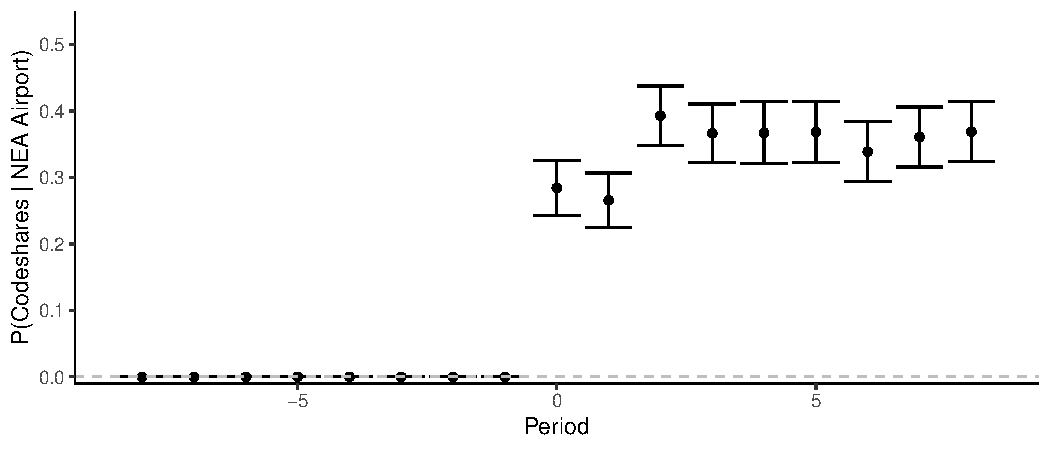
\includegraphics[width =\linewidth]{NEA_Probability_Switches_Graph}
		\footnotesize{Figure plots the estimated event study coefficients from Table \ref{tab:NEA_Switch_Prob}. Dependent variable is the probability that within a nonstop market, at least one passenger took planes operated by both American and JetBlue as part of their itinerary. Base period is 2021 Quarter 2. All data from 2020 and the first quarter of 2021 is excluded, as such,  Period -1 is the fourth quarter of 2019.}
        \end{center}
	\end{figure}

	As would be expected, no codesharing itineraries are booked before the start of the NEA and any market covered by it had approximately a 37\% chance of having codeshare routes following the implementation of the agreement. Beyond the numerical significance of these estimates, they help confirm the overall implementation timeline. The first two quarters of the alliance saw fewer markets with codesharing tickets than the other quarters. This is consistent with the implementation timeline of the agreement publicized in the press, with additional markets added to the codesharing agreement over time. As such, this reinforces the value of the increased observational period compared to past research which had data through the end of 2021. 
	
	I now turn my attention to identifying the effects of the NEA on airfare. Past literature on the aviation industry has generally used one of two outcomes of interest: either the average market fare or the average per-mile fare ("market yield").  While the literature has largely focused on fares in evaluating the effects of anti-competitive practices (such as in \citet{luo_price_2014, carlton_are_2019}), the only existing study \citep{zou_assessing_2023} to evaluate the NEA focused on yields as its variable of interest. As such, I estimate models with both fares and yields as outcomes to allow for easier comparison of my results with the past literature. 

    I model the average airfare $Y_{jt}$ for origin-destination pair $j$ in period $t$ as \[Y_{jt} = \alpha N_{j} + \sum_{T = -8}^{8} \delta_{T} P_{t = T} + \sum_{T = -8, t = 8} \gamma_{T} N_{j} P_{t = T} + \beta X_{jt} + \epsilon_{jt}\] where $N_{j}$ is a dummy variable if the market includes an endpoint covered by the NEA agreement, $P_{t = T}$ is a variable which is 1 if $t = T$ and 0 otherwise, $X_{jt}$ is a vector of additional market level controls which includes the log of the geometric mean income of the origin and destination metropolitan statistical areas, the log of the geometric mean population of the origin and destination metropolitan statistical areas, the lagged HHI for these markets, state coronavirus rates, the lagged share of nonstop flights, and the lagged average distance traveled within the market. Finally, $\epsilon_{jt}$ is a random error term. 

    These results are plotted in Figure \ref{fig:NEA_Market_Fare}. As is evident in the figure, the presence of substantial pre-trends suggests that the differences-in-differences inference strategy is invalid to use here. However, adding additional airport interaction terms for the each airports covered by the NEA agreement removes the pre-trends for both of Boston Logan International Airport (BOS) and Newark Liberty International Airport (EWR). These results are depicted in Figure \ref{fig:NEA_Airport_Fare_Interaction}. It appears that the NEA increased fares at BOS and decreased fares at EWR. That the estimated coefficients for Newark are negative is consistent with the evidence from Table \ref{tab:NEA_Airport_Prescence} that markets with Newark as the originating airport had the least overlap between the carriers before the agreement, suggesting that the potential for anti-competitive effects from the alliance was limited. 


    \begin{figure}
		\caption{NEA Market Fare - Airport Interaction Results}
		\label{fig:NEA_Airport_Fare_Interaction}
		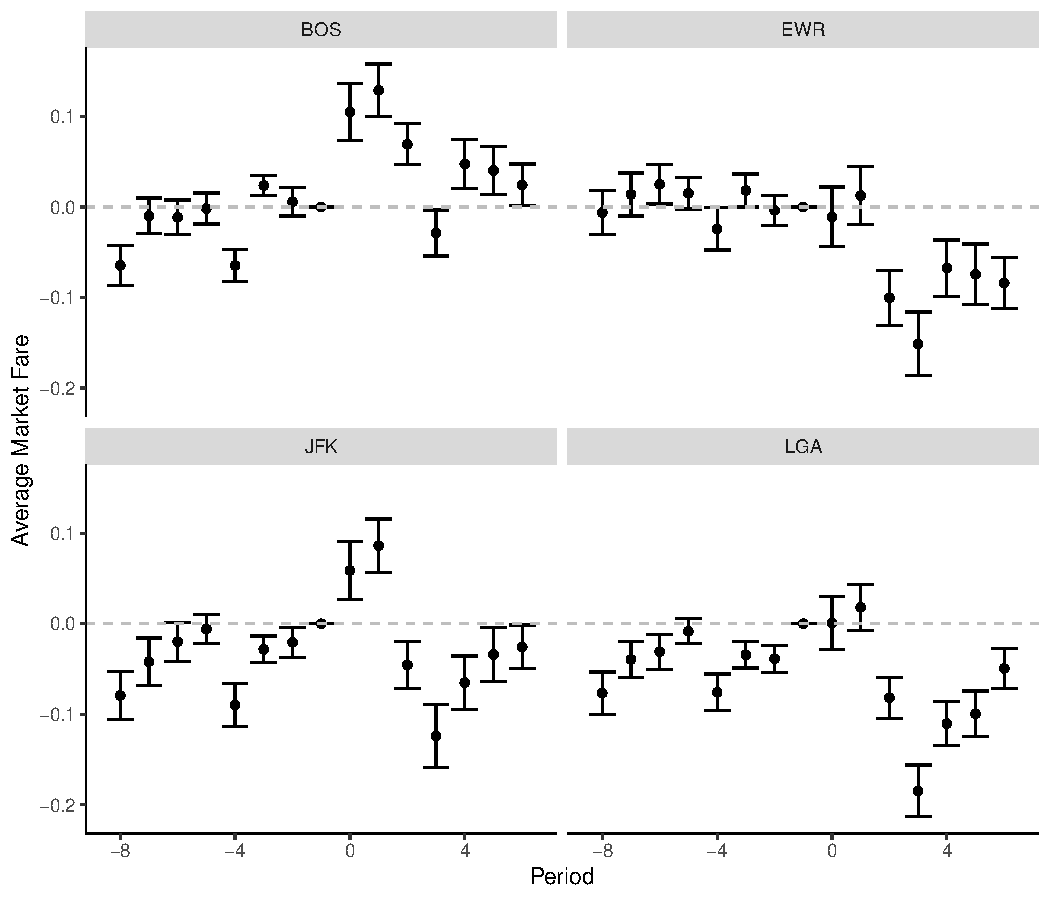
\includegraphics[width = \linewidth]{NEA_Airport_Fare_Graph}
		\footnotesize{Coefficients from a model based on the model reported in Table \ref{tab:NEA_Market_Fare} but which includes airport-time interaction terms are reported. Base period is 2021 Quarter 2. All data from 2020 and the first quarter of 2021 is excluded, and as such, Period -1 is the fourth quarter of 2019. Standard errors clustered at the level of origin-destination pairs are reported. }
	\end{figure}
    
	% I now turn my attention to the difference in average fares within markets with itineraries listing both airlines as the ticketing carrier. The results for this estimation are contained in Table \ref{tab:NEA_Fare_Neutral} and graphed in Figure \ref{fig:NEA_Fare_Neutral}.\footnote{Results for the average market yield are included in Table \ref{tab:NEA_Yield_Neutral} and Figure \ref{fig:NEA_Yield_Neutral} and follow the same trend.} I estimate that after the third quarter of the NEA's operation, this difference was consistently lower by about \$75 dollars within markets impacted by the NEA. This decline is consistent with the collaborating firms' stated desire for consumers to treat products offered by each firm as neutral and the timeline is consistent with my results in Table \ref{tab:NEA_Switch_Prob}. I fail to observe evidence of pre-trends, lending credence to the argument that the NEA reduced the price spread between American and JetBlue tickets. However, this result does not clarify if this was caused by American fares becoming less expensive or JetBlue fares becoming more expensive. 	

\end{document}